\documentclass[12pt]{article}


\usepackage{graphicx}
\usepackage{fancyhdr}

\usepackage{listings}
\usepackage{hyperref}
\usepackage{amsmath} % added to define math text commands

\usepackage[utf8]{inputenc}
\usepackage[english]{babel}

\usepackage{a4wide}

\usepackage{blindtext}
\renewcommand{\baselinestretch}{1.25}  
\newcommand\crule[3][black]{\textcolor{#1}{\rule{#2}{#3}}}
 
\pagestyle{fancy}
\fancyhf{}
\rhead{Marc Gaspà Joval\\Raul Hidalgo Caballero}
\lhead{
\includegraphics[width=2.5cm]{logoudl.png}}
\setlength{\headheight}{30pt}

\fancyfoot[R]{\thepage}
\rfoot{\thepage}
\renewcommand{\footrulewidth}{0.4pt}
\setlength{\footskip}{25pt}


\graphicspath{{images/}}

\begin{document}
\begin{titlepage}
	\newcommand{\HRule}{\rule{\linewidth}{0.5mm}}

	\center

	
\includegraphics[width=5cm]{logoudl.png}\\
	\textsc{\Large MEINF}\\[0.5cm]
	\textsc{\large High Performance Computing}\\[0.5cm]

	\HRule\\[0.4cm]

	{\huge\bfseries HPC Project: Heat Diffusion Equation}\\[0.4cm]
	{\LARGE Second Delivery (Hybrid Implementation with OpenMP-MPI)}
	\HRule\\[1.5cm]

	\textsc{Marc Gaspà Joval\\Raul Hidalgo Caballero}

	\vfill\vfill\vfill
	{\large\today}
\end{titlepage}
\pagebreak
\thispagestyle{empty}
\tableofcontents
\pagebreak
\thispagestyle{empty}
\listoftables
\pagebreak

\section{Strategy}
From the two possible strategies, we used the \textbf{Static mapping of tasks} strategy. The main reason we chose this approach is that it is faster to implement and easier to understand.

\subsection{Static mapping of tasks}
In our case, we have a 2D grid of	 size $N \times N$, and we want to divide it into $P$ subgrids, which correspond to the number of slots we will allocate in the cluster.
\\\\
Although the image in the assignment suggests dividing into square subgrids, we decided to divide the grid into rectangular subgrids. This choice allows for better memory locality and improved cache usage.

\begin{figure}[h!]
	\centering
	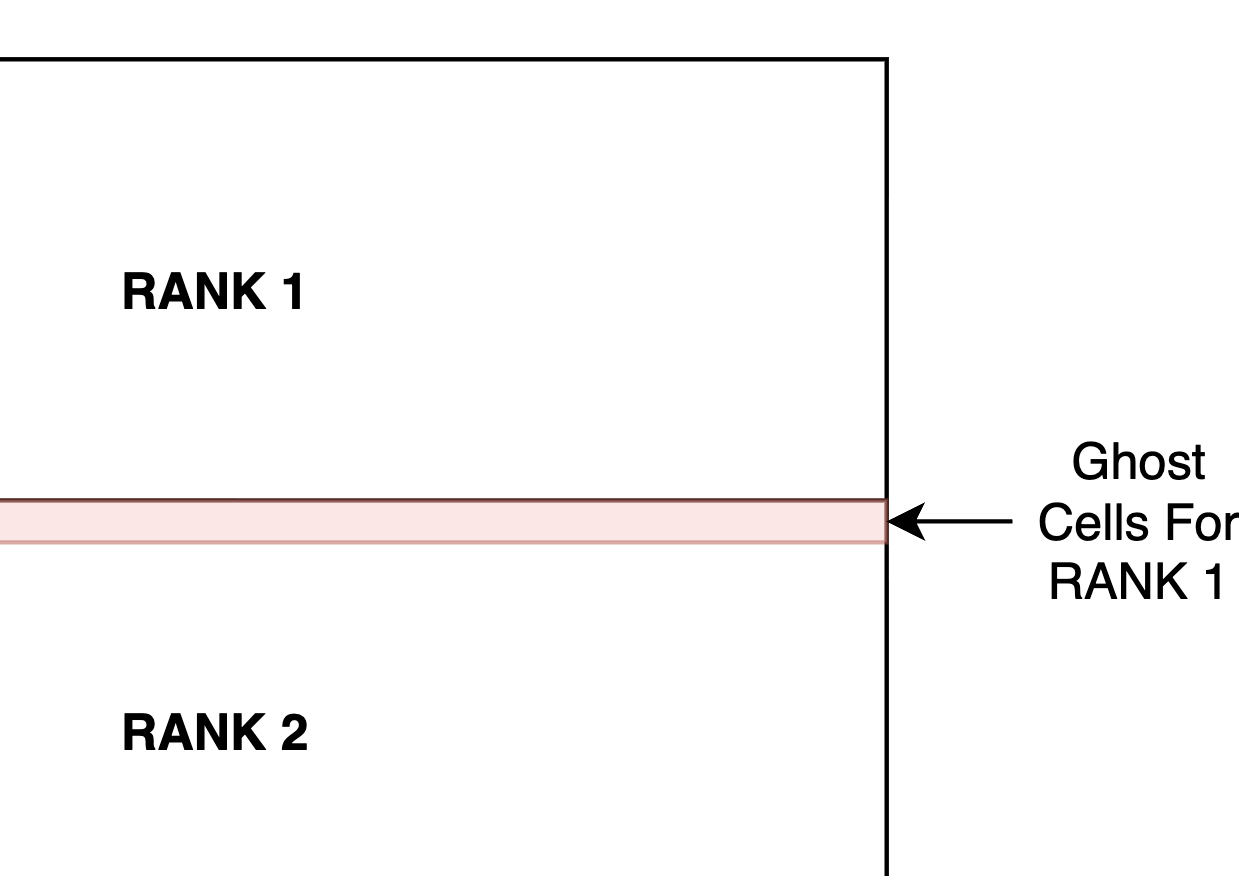
\includegraphics[width=0.8\textwidth]{ghost_cells.png}
	\caption{Illustration of the grid division into rectangular subgrids. And the ghost cells that are used to communicate with the neighbors.}
	\label{fig:grid_division}
\end{figure}

\newpage
\subsection{Communication}
In our implementation, communication is performed at three key stages:

\begin{itemize}
	\item \textbf{Initialization:} Each process must receive its portion of the global grid, including two extra rows (ghost rows) for neighbor data. This is achieved using \texttt{MPI\_Scatterv}, which distributes variable-sized blocks of data to each process.

	\item \textbf{Iteration:} At the beginning of each iteration, processes exchange boundary rows with their neighbors to update ghost rows. This is done using \texttt{MPI\_Isend} and \texttt{MPI\_Irecv} for non-blocking communication, followed by \texttt{MPI\_Waitall} to ensure all communications complete before proceeding with computation.

	\item \textbf{Finalization:} Once computation is complete, each process sends its subgrid back to the master process. We use \texttt{MPI\_Gatherv} to collect variable-sized subgrids and reconstruct the full grid in the master process before writing it to a file.
\end{itemize}

\newpage
\subsection{Load Balancing}
Load balancing is not a concern in our case since the number of iterations and the number of grid cells are fixed. To ensure an even workload distribution, we divide the grid into rectangular subgrids of nearly equal size among the processes.
\\\\
One limitation is that we do not currently handle the case where the grid size is not divisible by the number of processes. In such scenarios, the last part of the grid may lose some rows. This could be improved by implementing a remainder handling strategy in the grid division.



\newpage
\section{Scalability of the Program}

\subsection{Performance Measurement Methodology}

In this case, as we re using MPI, we will use the \texttt{MPI\_Wtime} function to measure the time taken by each process.

\subsection{Performance Metrics and Their Formulas}


\begin{table}[h!]
	\centering
	\begin{tabular}{lcccc}
		\hline
		\textbf{Matrix Size} & \multicolumn{4}{c}{\textbf{Steps}}                                                    \\
		\cline{2-5}
		                     & \textbf{100}                       & \textbf{1000} & \textbf{10000} & \textbf{100000} \\
		\hline
		$100\times 100$      & 0.010000s                          & 0.100000s     & 1.080000s      & 10.820000s      \\
		$1000\times 1000$    & 1.200000s                          & 12.780000s    & 119.870000s    & 1070.680000s    \\
		$2000\times 2000$    & 4.750000s                          & 47.630000s    & 503.060000s    & 4310.300000s    \\
		\hline
	\end{tabular}
	\caption{Execution times of the \texttt{heat\_serial} program.}
	\label{tab:serial_times}
\end{table}

\newpage
\begin{table}[h!]
	\centering
	\begin{tabular}{lcccc}
		\hline
		\textbf{Nodes: 2} & \multicolumn{4}{c}{\textbf{Steps}}                                                    \\
		\cline{2-5}
		                  & \textbf{100}                       & \textbf{1000} & \textbf{10000} & \textbf{100000} \\
		\hline
		$1000\times 1000$ & 3.226295s                          & 28.773441s    & 269.608456s    & 2451.152783s    \\
		$100\times 100$   & 3.008608s                          & 30.182583s    & 151.455907s    & 997.242430s     \\
		$2000\times 2000$ & 4.463269s                          & 42.416510s    & 323.633867s    & 2576.611911s    \\
		\hline
	\end{tabular}
	\caption{Execution times of the \texttt{heat\_parallel} hybrid program with 2 nodes.}
	\label{tab:mpi_times_2_nodes}
\end{table}

\begin{table}[h!]
	\centering
	\begin{tabular}{lcccc}
		\hline
		\textbf{Nodes: 4} & \multicolumn{4}{c}{\textbf{Steps}}                                                    \\
		\cline{2-5}
		                  & \textbf{100}                       & \textbf{1000} & \textbf{10000} & \textbf{100000} \\
		\hline
		$1000\times 1000$ & 3.466167s                          & 32.299433s    & 318.805040s    & 3184.036661s    \\
		$100\times 100$   & 2.661267s                          & 26.713319s    & 372.033094s    & 2572.231210s    \\
		$2000\times 2000$ & 5.508030s                          & 47.554560s    & 437.503118s    & 3524.018770s    \\
		\hline
	\end{tabular}
	\caption{Execution times of the \texttt{heat\_parallel} hybrid program with 4 nodes.}
	\label{tab:mpi_times_4_nodes}
\end{table}

\begin{table}[h!]
	\centering
	\begin{tabular}{lcccc}
		\hline
		\textbf{Nodes: 5} & \multicolumn{4}{c}{\textbf{Steps}}                                                    \\
		\cline{2-5}
		                  & \textbf{100}                       & \textbf{1000} & \textbf{10000} & \textbf{100000} \\
		\hline
		$1000\times 1000$ & 2.874023s                          & 27.269382s    & 382.538333s    & 3183.711562s    \\
		$100\times 100$   & 2.222764s                          & 23.600960s    & 310.150252s    & 3098.737703s    \\
		$2000\times 2000$ & 4.407035s                          & 36.218476s    & 428.217962s    & 3336.180224s    \\
		\hline
	\end{tabular}
	\caption{Execution times of the \texttt{heat\_parallel} hybrid program with 5 nodes.}
	\label{tab:mpi_times_5_nodes}
\end{table}

\newpage
\subsection{Speedup and Efficiency}
Speedup formula:
\begin{equation}
	S = \frac{T_{serial}}{T_{parallel}}
\end{equation}

\begin{table}[h!]
	\centering
	\begin{tabular}{lccccc}
		\hline
		\textbf{Matrix Size} & \textbf{Threads} & \multicolumn{4}{c}{\textbf{Steps}}                                                    \\
		\cline{3-6}
		                     &                  & \textbf{100}                       & \textbf{1000} & \textbf{10000} & \textbf{100000} \\
		\hline
		$100\times 100$      & 2                & 0.003324                           & 0.003313      & 0.007131       & 0.010850        \\
		                     & 4                & 0.003758                           & 0.003743      & 0.002903       & 0.004206        \\
		                     & 5                & 0.004499                           & 0.004237      & 0.003482       & 0.003492        \\
		$1000\times 1000$    & 2                & 0.371944                           & 0.444160      & 0.444608       & 0.436807        \\
		                     & 4                & 0.346204                           & 0.395673      & 0.375998       & 0.336265        \\
		                     & 5                & 0.417533                           & 0.468657      & 0.313354       & 0.336299        \\
		$2000\times 2000$    & 2                & 1.064242                           & 1.122912      & 1.554411       & 1.672856        \\
		                     & 4                & 0.862377                           & 1.001586      & 1.149843       & 1.223121        \\
		                     & 5                & 1.077822                           & 1.315075      & 1.174776       & 1.291987        \\
		\hline
	\end{tabular}
	\caption{Speedup of the parallel program with respect to the serial one for different thread counts.}
	\label{tab:speedup}
\end{table}


\begin{figure}[h!]
	\centering
	
\includegraphics[width=0.8\textwidth]{mpi_speedup.png}
	\caption{Scalability analysis of the program for different matrix sizes and thread counts.}
	\label{fig:scalability_plot}
\end{figure}

\newpage
Efficiency formula:
\begin{equation}
	E = \frac{S}{P}
\end{equation}
Here, $P$ represents the number of processes utilized. We used 2, 4, and 5 processes for our tests.

\begin{table}[h!]
	\centering
	\begin{tabular}{lccccc}
		\hline
		\textbf{Matrix Size} & \textbf{Threads} & \multicolumn{4}{c}{\textbf{Steps}}                                                    \\
		\cline{3-6}
		                     &                  & \textbf{100}                       & \textbf{1000} & \textbf{10000} & \textbf{100000} \\
		\hline
		$100\times 100$      & 2                & 0.001662                           & 0.001657      & 0.003565       & 0.005425        \\
		                     & 4                & 0.000939                           & 0.000936      & 0.000726       & 0.001052        \\
		                     & 5                & 0.000900                           & 0.000847      & 0.000696       & 0.000698        \\
		$1000\times 1000$    & 2                & 0.185972                           & 0.222080      & 0.222304       & 0.218403        \\
		                     & 4                & 0.086551                           & 0.098918      & 0.093999       & 0.084066        \\
		                     & 5                & 0.083507                           & 0.093731      & 0.062671       & 0.067260        \\
		$2000\times 2000$    & 2                & 0.532121                           & 0.561456      & 0.777205       & 0.836428        \\
		                     & 4                & 0.215594                           & 0.250397      & 0.287461       & 0.305780        \\
		                     & 5                & 0.215564                           & 0.263015      & 0.234955       & 0.258397        \\
		\hline
	\end{tabular}
	\caption{Efficiency of the parallel program with respect to the serial one for different thread counts.}
	\label{tab:efficiency}
\end{table}

\begin{figure}[h!]
	\centering
	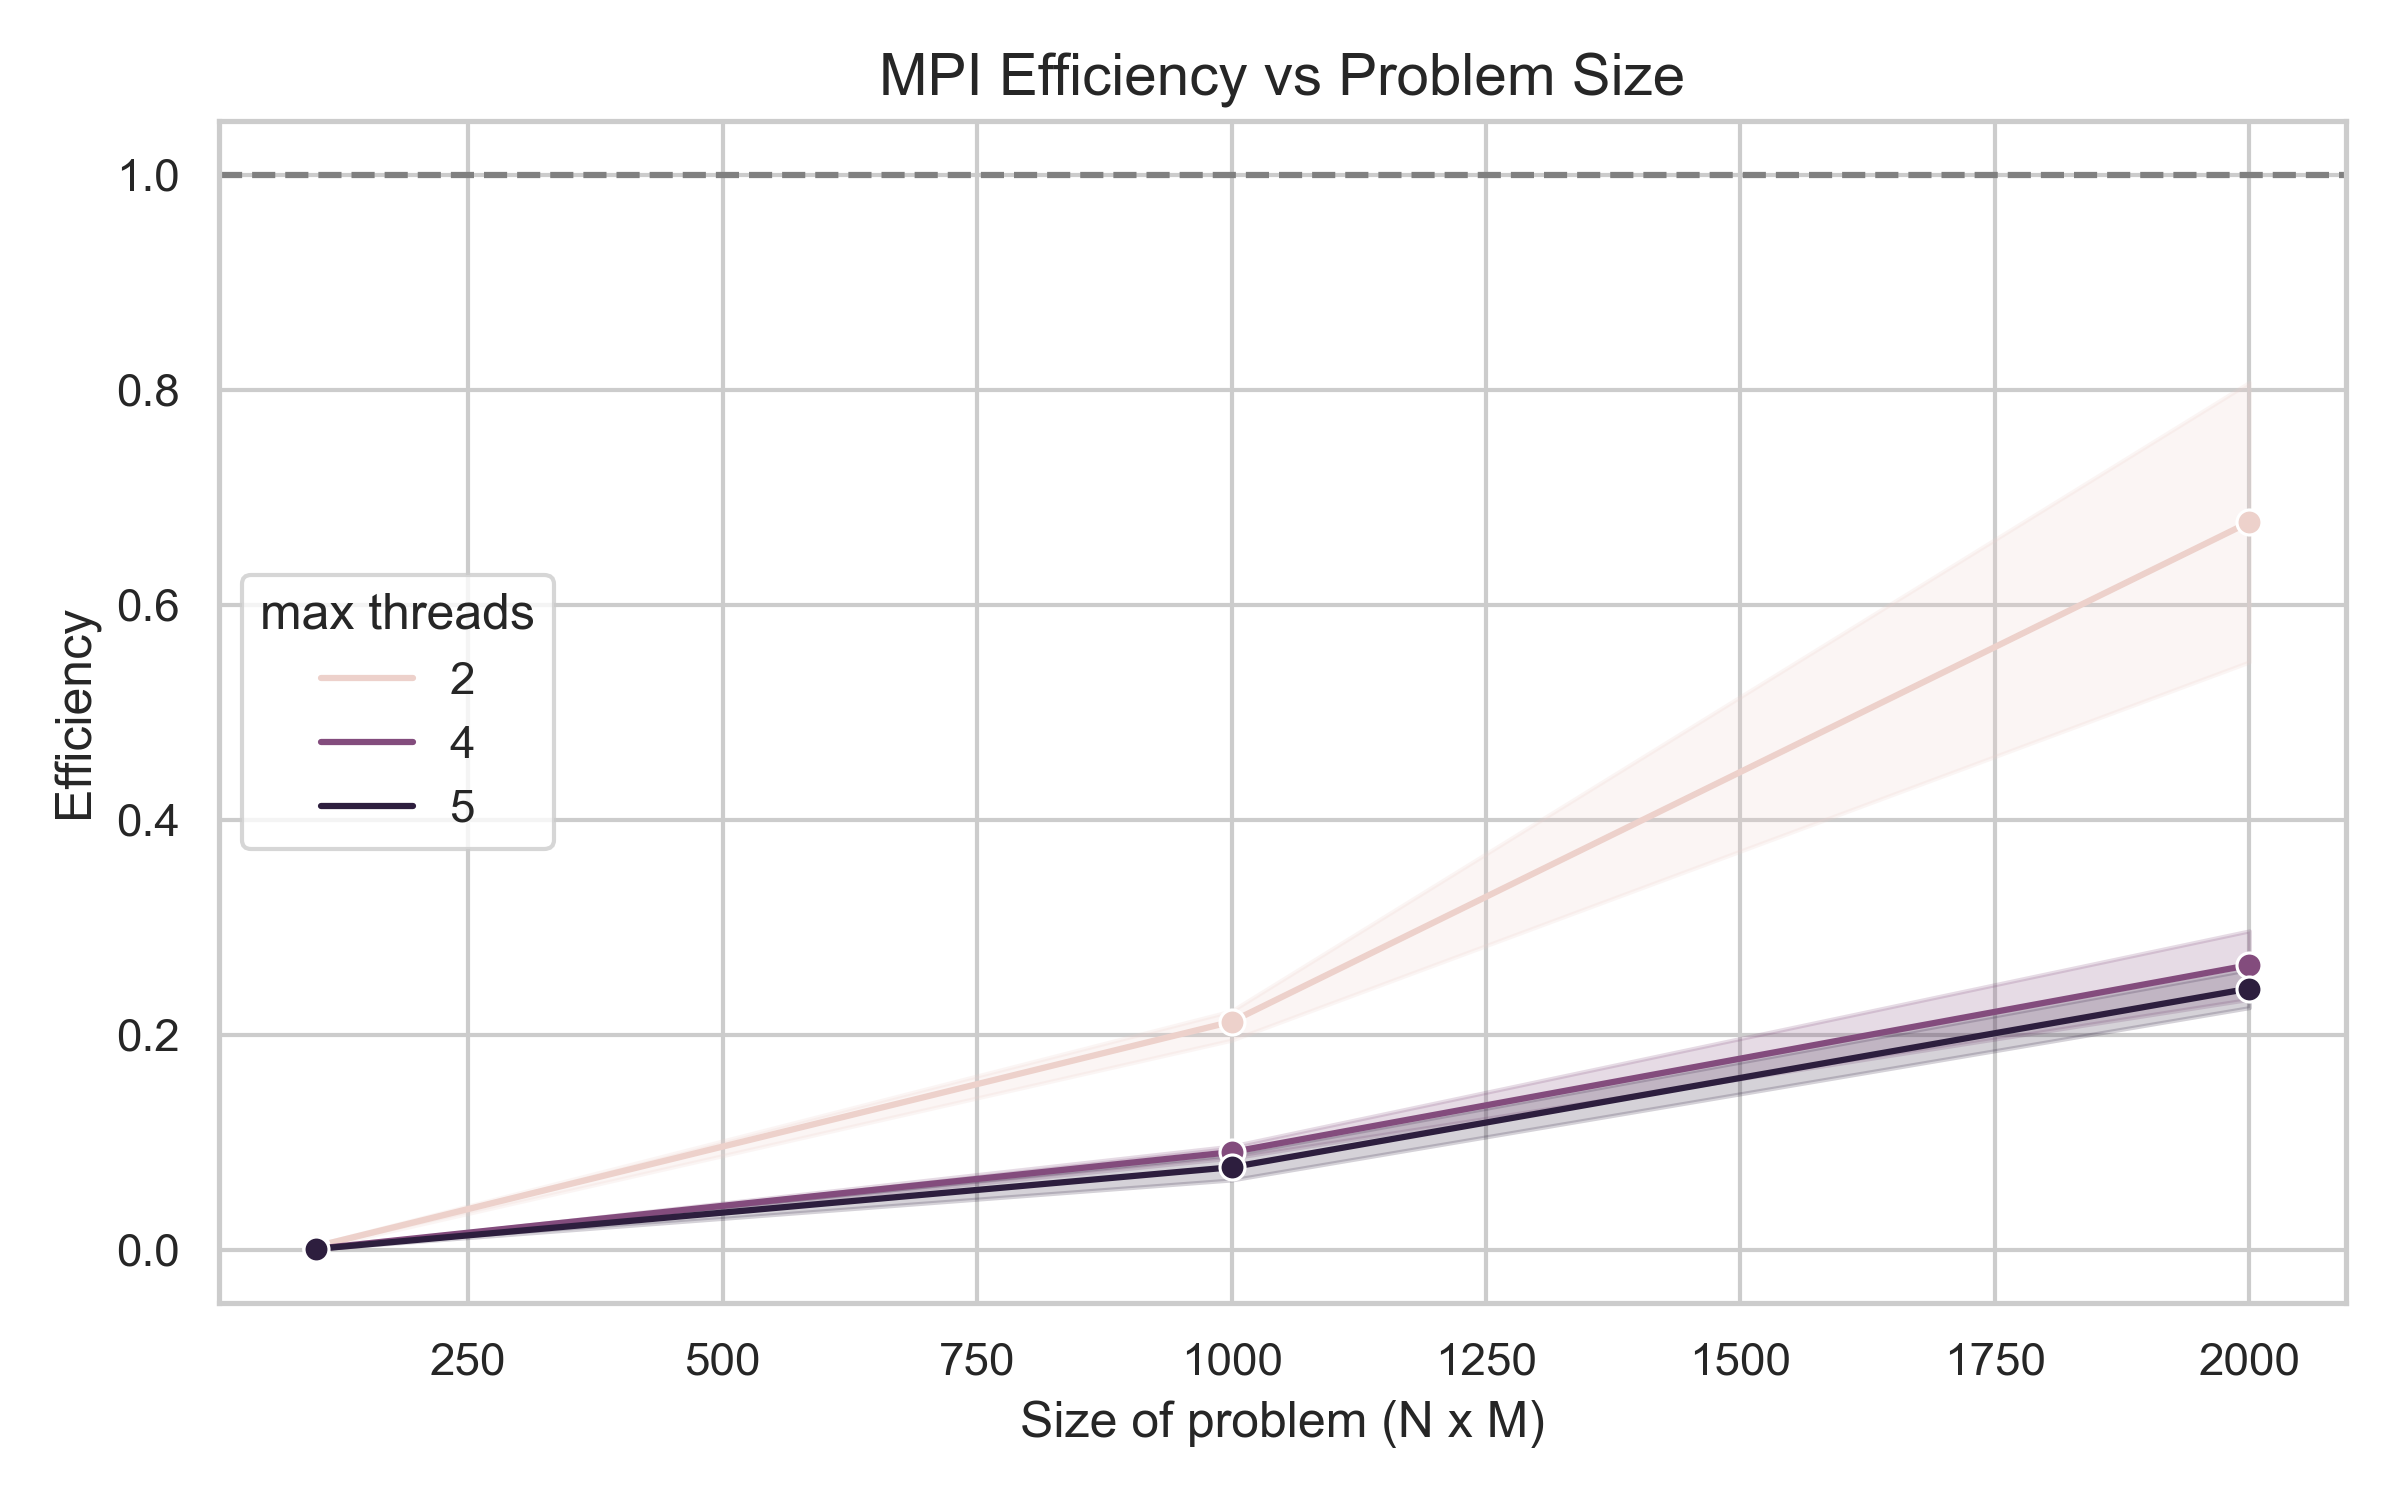
\includegraphics[width=0.8\textwidth]{mpi_efficiency.png}
	\caption{Efficiency analysis of the program for different matrix sizes and thread counts.}
	\label{fig:efficiency_plot}
\end{figure}

\subsection{Overhead Analysis}

As you can see in the previous data, the overhead in our implementation is important, only seeing speedups over 1 after the 2000x2000 matrix. This is because the overhead of the communication is greater than the time spent in the computation.\\\\
We will calculate the overhead using the following formula:
\begin{equation}
	O = \frac{T_{parallel} \cdot P - T_{serial}}{T_{parallel} \cdot P} \cdot 100
\end{equation}
Which is normalized to 100\% and gives us the percentage of time spent in communication.
\newpage
\begin{table}[h!]
	\centering
	\begin{tabular}{lccccc}
		\hline
		\textbf{Matrix Size} & \textbf{Threads} & \multicolumn{4}{c}{\textbf{Steps}}                                                    \\
		\cline{3-6}
		                     &                  & \textbf{100}                       & \textbf{1000} & \textbf{10000} & \textbf{100000} \\
		\hline
		$100\times 100$      & 2                & 0.060072                           & 0.602652      & 3.018318       & 19.836649       \\
		                     & 4                & 0.106351                           & 1.067533      & 14.870524      & 102.781048      \\
		                     & 5                & 0.111038                           & 1.179048      & 15.496713      & 154.828685      \\
		$1000\times 1000$    & 2                & 0.005253                           & 0.044767      & 0.419347       & 3.831626        \\
		                     & 4                & 0.012665                           & 0.116418      & 1.155350       & 11.665467       \\
		                     & 5                & 0.013170                           & 0.123567      & 1.792822       & 14.847878       \\
		$2000\times 2000$    & 2                & 0.002088                           & 0.018602      & 0.072104       & 0.421462        \\
		                     & 4                & 0.008641                           & 0.071294      & 0.623476       & 4.892888        \\
		                     & 5                & 0.008643                           & 0.066731      & 0.819015       & 6.185301        \\
		\hline
	\end{tabular}
	\caption{Overhead percentage of the parallel program for different thread counts and matrix sizes (normalized).}
	\label{tab:overhead}
\end{table}
\begin{figure}[h!]
	\centering
	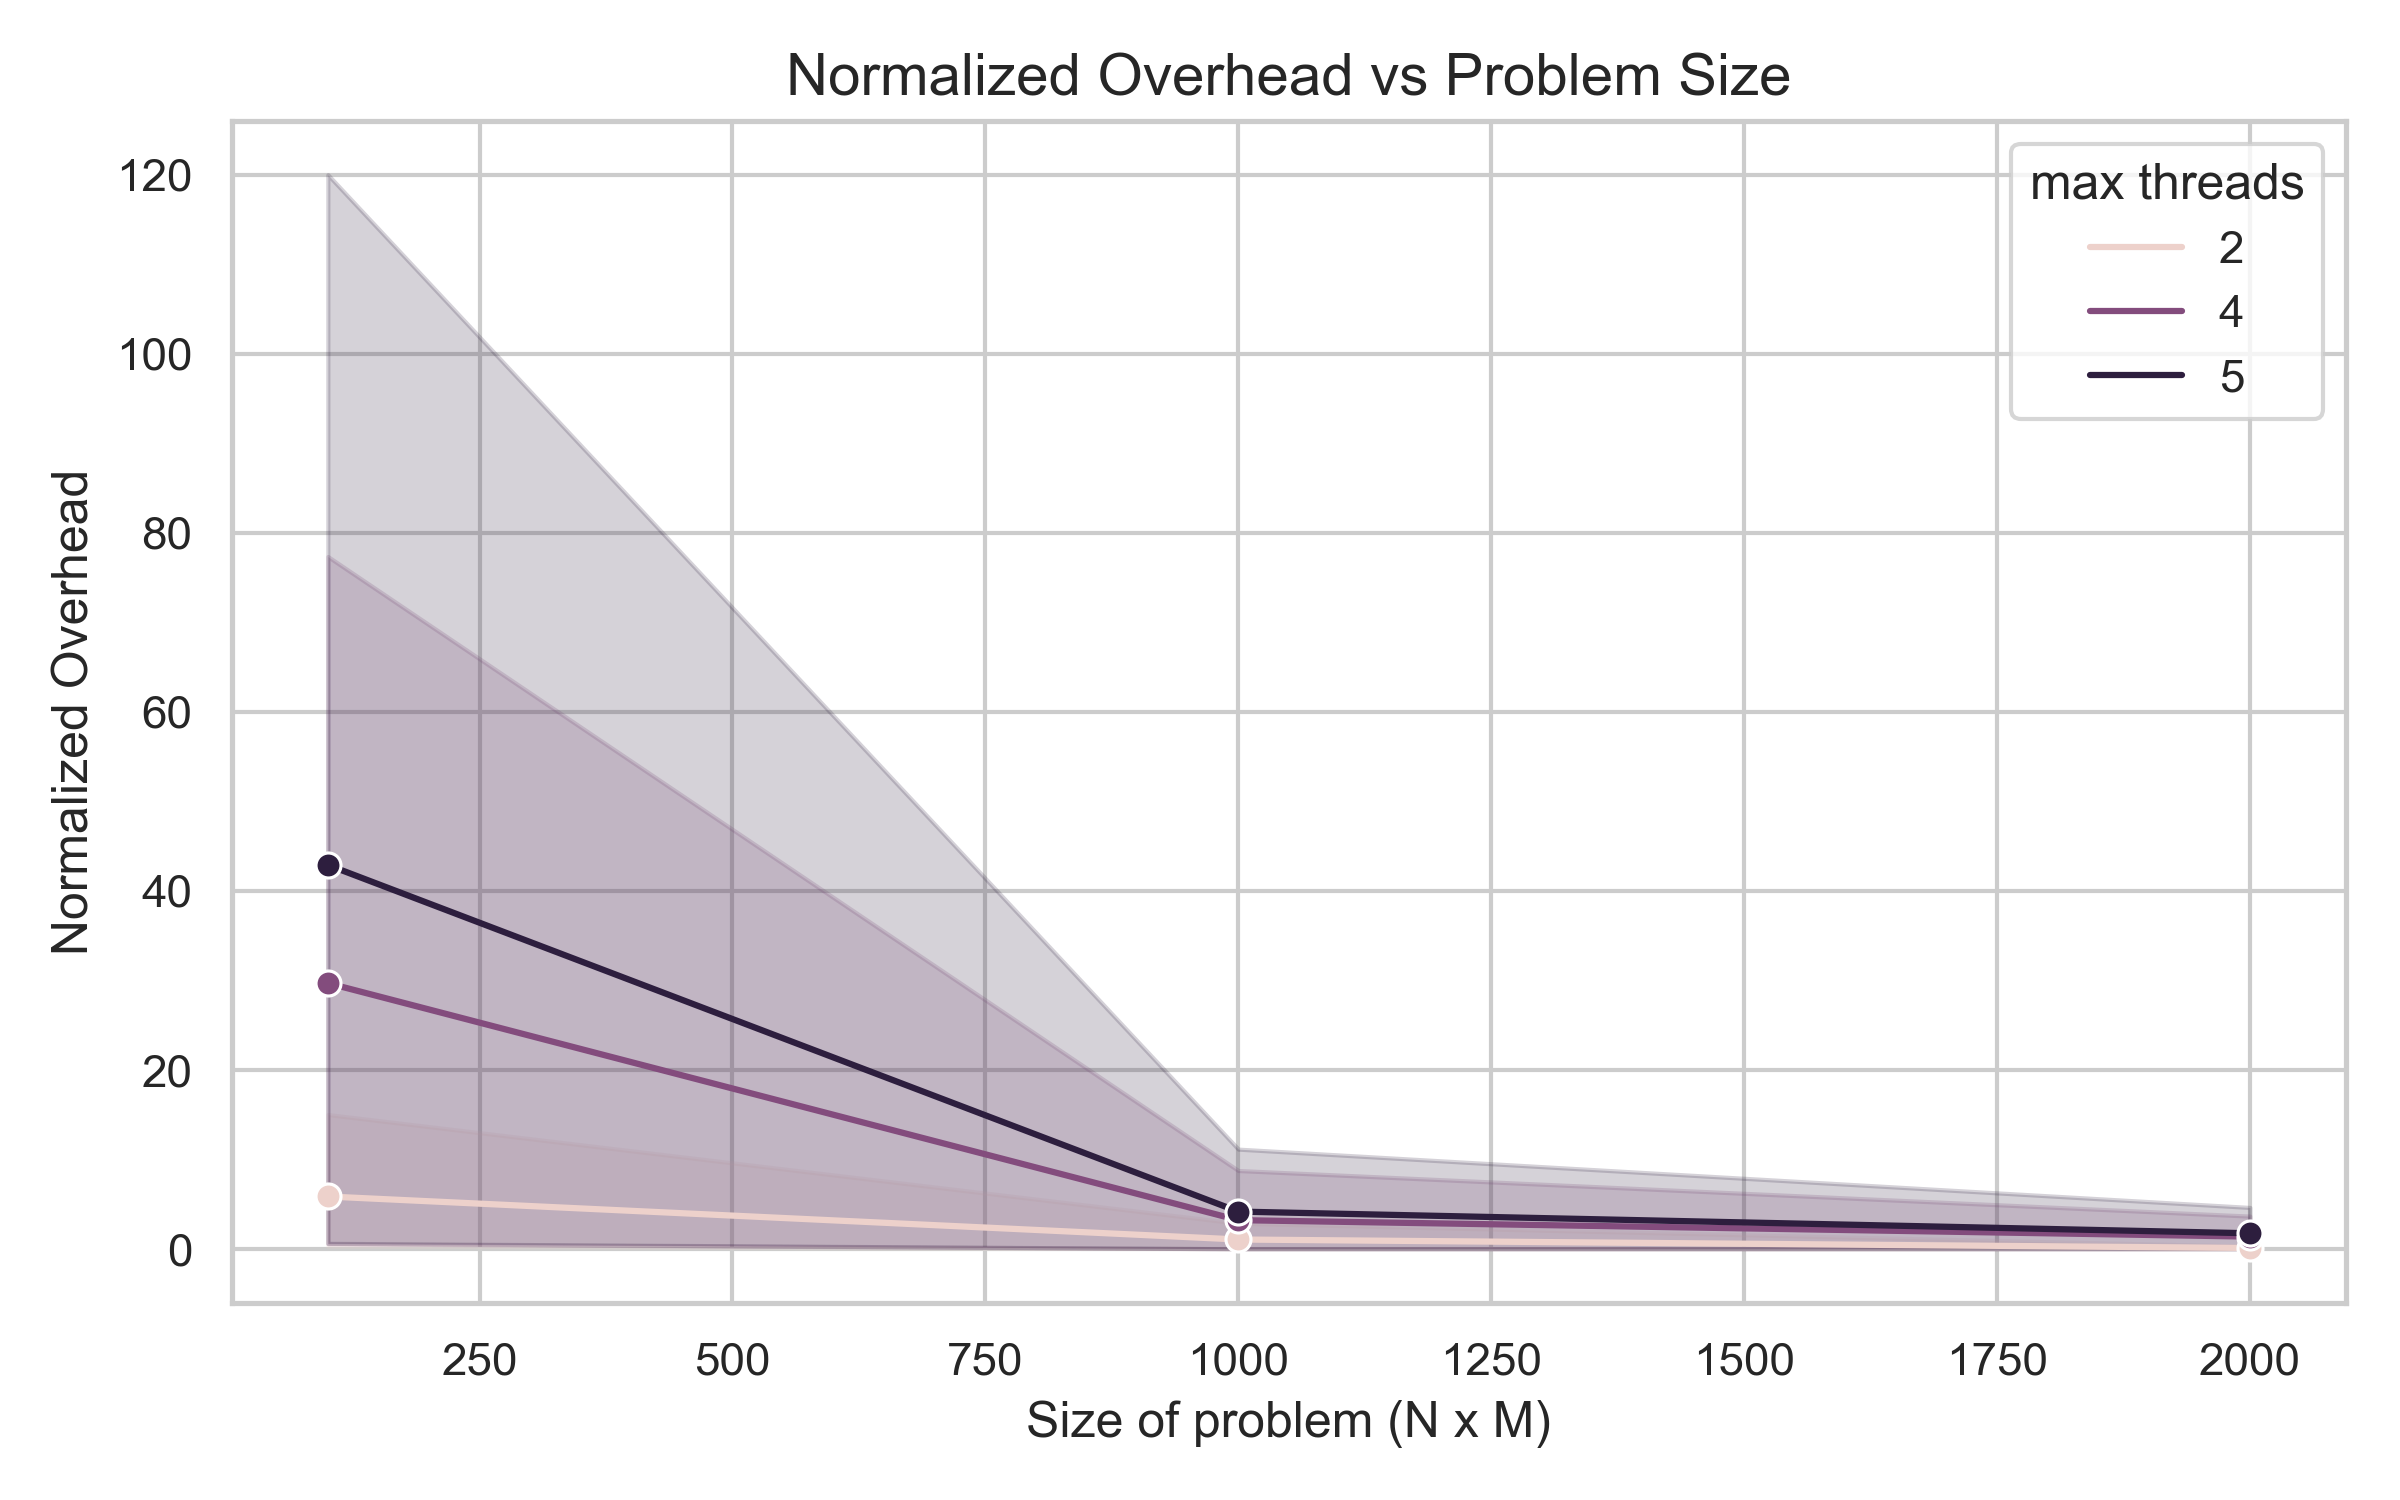
\includegraphics[width=0.8\textwidth]{normalized_overhead.png}
	\caption{Overhead analysis of the program for different matrix sizes and thread counts.}
	\label{fig:overhead_plot}
\end{figure}
\noindent
As we can see in the table and image, the overhead is very high for small matrix sizes, but it decreases as the matrix size increases. This is because the time spent in communication is less than the time spent in computation.

\end{document}